\chapter{Немного истории}

Эликсир молодой язык, он создан в 2012 году. Но начать я хочу за 100 лет до этого. 

\section{Предыстория: начало ХХ века.}

В начале ХХ века в Дании, в Копенгагенской телефонной компании работал инженер \href{https://ru.wikipedia.org/wiki/%D0%AD%D1%80%D0%BB%D0%B0%D0%BD%D0%B3,_%D0%90%D0%B3%D0%BD%D0%B5%D1%80_%D0%9A%D1%80%D0%B0%D1%80%D1%83%D0%BF}{Агнер Краруп Эрланг}

\begin{figure}[h]
  \centering
  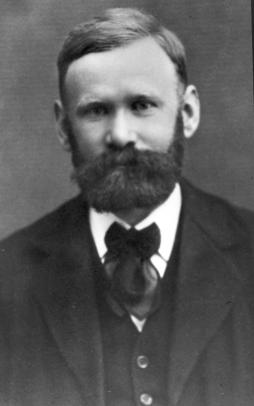
\includegraphics[width=0.3\textwidth]{./lesson_02/img/agner_krarup_erlang.jpg}
  \caption{Agner Krarup Erlang}
\end{figure}

Его интересовало, как наиболее эффективным образом использовать оборудование телефонной станции, чтобы обслуживать максимальное количество абонентов.

Агнер Эрланг был хорошо образован, с отличием закончил университет, и умел применять в работе методы математики и статистики. И он не ленился самостоятельно залезать на телефонные столбы, чтобы собрать нужные данные.

Результатом его усилий стала научная работа \href{https://ru.wikipedia.org/wiki/%D0%A2%D0%B5%D0%BE%D1%80%D0%B8%D1%8F_%D0%BC%D0%B0%D1%81%D1%81%D0%BE%D0%B2%D0%BE%D0%B3%D0%BE_%D0%BE%D0%B1%D1%81%D0%BB%D1%83%D0%B6%D0%B8%D0%B2%D0%B0%D0%BD%D0%B8%D1%8F}{"Теория массового обслуживания"}. Она позволяет рационально расчитать ресурсы, необходимые для обслуживания требований, поступающих в систему, исходя из длительности ожидания и длины очередей.

Теория применяется не только в телекоммуникационных системах, а гораздо шире: в управлении автомобильным и воздушным движением, на конвейерном производстве, в логистике, а также при проектировании фабрик, складов, магазинов и больниц.

В честь Агнера Эрланга названы единица измерения трафика в телекоммуникационных системах и язык программирования.

\section{История Эрланг: c 1985 по настоящее время.}

\begin{figure}[h]
  \centering
  
\includegraphics[width=0.3\textwidth]{./lesson_02/img/erlang_logo.png}
  \caption{Erlang}
\end{figure}

Язык \textbf{Эрланг} родился в недрах шведской компании Эрикссон (Ericsson) -- крупного поставщика телекомуникационного оборудования и услуг.

Для этой индустрии характерны сложное оборудование, сложный софт, большой траффик и жесткие требования по доступности сервиса.

В компании был отдел, занимающийся научной работой: \textit{Ericsson’s Computer Science Laboratory}. Отделу была поставлена задача найти более эффективные средства разработки софта для железа и сервисов компании.

У компании уже был опыт разработки языков программирования. Использовались собственные проприетарные языки \textit{PLEX} и \textit{EriPascal}. Но они не стремились разработать еще один язык, а хотели найти подходящее решение среди уже существующих.

В течение 2х лет отдел писал прототипы телеком-приложений на разных языках, имеющихся в то время:
\begin{itemize}
\item функциональные языки \textit{ML} и \textit{Miranda};
\item многопоточные языки \textit{ADA}, \textit{Modula} и \textit{Chill};
\item логический язык \textit{Prolog};
\item объектно-ориентированный \textit{Smalltalk}.
\end{itemize}

Разработчики пришли к выводу, что ни один язык не имеет нужных возможностей. И главная проблема была в реализации многопоточности на нужном уровне. В итоге лаборатория решила разработать свой язык программирования.

В отличие от большинства языков, разработанных для "общего" применения и на "правильном" теоретическом базисе, Эрланг изначально разрабатывался для узкого применения, исходя из практических требований. От этого идут его преимущества и недостатки.

В 1998 Эрланг был выпущен в open source, и стал известен за пределами Эрикссон. Следующие несколько лет он использовался в Эрикссон, и отдельными энтузиастами за пределами компании, но был мало известен.

В 2002 году был начат проект \textbf{ejabberd} -- первый крупный open source проект на Эрланг. Он стал основой для большинства IM (Instant Messaging) систем, в т.ч. для широко известного \textbf{WhatsApp}.

В 2006 году в появилась поддержка симметричной мультипроцессорности (SMP). Эрланг научился эффективно использовать все имеющиеся в системе процессорные ядра.

И это случилось в подходящий момент. К этому времени производители процессоров достигли предела тактовых частот. Дальше наращивать мощность одного процессора было невозможно, и производители пошли по пути увеличения числа процессоров.

А у IT-индустрии появилась потребность разрабатывать многопоточные программы, эффективно использующие несколько процессоров. Делать это на популярных языках программирования было трудно, и возник интерес к функциональному программированию вообще, и к Эрланг в частности.

Этот интерес проявился в двух направлениях:
\begin{itemize}
\item стали шире использоваться ФП языки;
\item популярные языки начали заимствовать идеи ФП и реализовывать их у себя.
\end{itemize}

В 2007 вышла книга Джо Армстронга "Programming Erlang".

Нынче Эрланг известен и применяется достаточно широко.

\section{История Эликсир: c 2012 по настоящее время.}

\begin{figure}[h]
  \centering
  
\includegraphics[width=0.3\textwidth]{./lesson_02/img/elixir_logo.png}
  \caption{Elixir}
\end{figure}

\textbf{Эликсир} создан в 2012 году как исследовательский проект в компании Plataformatec. Его автор -- \textbf{Жозе Валим}, был одним из основных разработчиков фреймворка \textit{Ruby on Rails} и сооснователем компании \textit{Plataformatec}.

Авторы языка имели большой опыт веб-разработки на разных языках и с разными фреймворками. Как это обычно бывает, они постарались собрать в одном языке все лучшее из своего опыта.

Эликсир позаимствовал идеи из Ruby, Clojure и Эрланг. Большое влияние оказали Ruby и фрейморк Ruby on Rails. Система макросов заимствована из Clojure. Ну и, конечно, Эликсир унаследовал все возможности Эрланг и его виртуальной машины.

Почти одновременно с Эликсир создавались \textit{Ecto} -- библиотека для работы с реляционными базами данных и фреймворк \textit{Phoenix}.

Первая версия языка вышла в 2014 году. Немного позже, в 2015 году, вышли первые версии Ecto и Phoenix. С тех пор язык и библиотеки активно развиваются. Вокруг них сформировалось большое сообщество.
